Hay dos obras importantes en matemática: una es los Nueve Capítulos y la otra, los Diez Cánones del Cálculo. Los Nueve Capítulos es una recolección de problemas, muchos de ellos son de origen geométrico. En estos se ve cuáles son las preocupaciones en China: repartos, construcciones. En los Diez Cánones del Cálculo se describen los diversos sistemas de numeración que tienen: unos de comercio, otros de contabilidad, unos posicionales y otros no. Depende la situación a resolver, se usaba un sistema por sobre los otros. Manejan números positivos y negativos. Los positivos los escriben en rojo y los negativos en negro, porque el rojo corresponde a la abundancia. Las cuentas las hacen con ábacos (de palitos y bolitas), que se sigue utilizando en la actualidad.
Además de los número enteros, trabajaban con números con cifras decimales y no se preocupaban por saber si eran racionales o irracionales, no tenían ese concepto, simplemente trabajaban con aproximaciones tan grandes como les era necesario.

Tienen un teorema llamado de Kou Ku. Significa "lado largo" y se refiere a un cuadrado construido sobre un lado largo de un triángulo, que es suma de los cuadrados de los lados más cortos. El método de demostración estaba basado en la contemplación: dado un teorema se contemplaba, si no se encontraba contradicción, quedaba demostrado. Por eso las demostraciones eran gráficas: si el movimiento de las piezas era el adecuado, estaba demostrado. En China no hubo demostraciones deductivas.

Algo que también se encontraba en grabados chinos es el triángulo de Pascal. La utilidad que le daban no es la misma que la actual de número combinatorio o desarrollo de potencias, trabajaban algo similar al binomio de Newton, cuando necesitaban multiplicar números, los dividían en dos sumandos y trabajaban desde esos sumandos, es decir, hacían una especie de desarrollo utilizando el triángulo. Es el método que posteriormente va a descubrir/crear Gauss a principios del siglo XIX.

Desarrollaron el principio de complementariedad interna y externa, que es lo que se conoce hoy en día como el principio de conservación de áreas y volúmenes: si yo tengo una figura con cierta área obtenida como suma de ciertas piezas, por más que yo cambie su forma, se va a mantener. Eso se refleja, por ejemplo, en los rompecabezas, el tangram (actualmente se le ha dado finalidades didácticas, originalmente era para entretenimiento). 

Este principio es utilizado con volúmenes, trabajando a partir del cubo. Por ejemplo, si se tiene un cubo de volumen V, se puede considerar una parte de ese cubo, digamos su mitad. Esto era un Qiandu. También definieron un tercio del volumen de un cubo (Yangma) y un sexto (Bienao).
\begin{center}
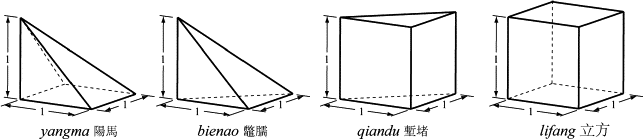
\includegraphics[scale=0.6]{all}
\end{center}
Agregando y quitando piezas pueden calcular diferentes volúmenes. Trabajaban de esa manera muchas veces, sumando y restando con el movimiento de piezas.
\begin{center}
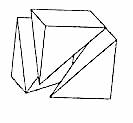
\includegraphics[scale=0.8]{image005.jpg}
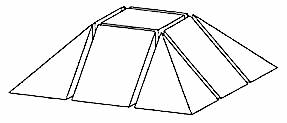
\includegraphics[scale=0.8]{image007.jpg}
\end{center}
En China sabían resolver raíces cuadradas y cúbicas y ecuaciones de primero y segundo grado. En algunos problemas trabajaban algo parecido a sucesiones, que las cortan, las terminan trabajando de manera finita. Pero aparece la idea de que se puede prolongar y trabajar más de esas sucesiones.

Su matemática es matemática aplicada, en función de resolver problemas. Aplicaron la matemática, por ejemplo, para concebir los cuadrados mágicos: cuadrados con cierta cantidad de cuadrículas, donde la suma de cada fila y cada columna corresponden a una constante. Dicen que el primer cuadrado mágico lo encuentra un pescador sobre la caparazón de una tortuga y a partir de ahí le empieza a ir bien, por lo que se construyen amuletos con cuadrados mágicos. Cuanto más grande, más suerte y más abundancia trae.
